\documentclass[runningheads]{llncs}

% OpenReview submission ID 11.
\usepackage[review,year=2026,ID=11]{accv}
\usepackage{accvabbrv}
\usepackage{booktabs}
\usepackage{graphicx}
\usepackage{microtype}
\usepackage{amsmath,amssymb}
\usepackage{xcolor}
\usepackage{multirow}
\usepackage{siunitx}
\usepackage[pagebackref,breaklinks,colorlinks,citecolor=accvblue]{hyperref}
\hypersetup{pdftitle={Supervising Both Views: Camera Robustness under Label Scarcity}}
\usepackage[capitalize,noabbrev]{cleveref}
\setlength{\emergencystretch}{1em}

% Pack floats a little tighter than the LNCS defaults.
\renewcommand{\topfraction}{0.92}
\renewcommand{\textfraction}{0.07}
\renewcommand{\floatpagefraction}{0.85}
\setlength{\textfloatsep}{9pt plus 2pt minus 3pt}
\setlength{\abovecaptionskip}{6pt}
\AtBeginDocument{%
\setlength{\abovedisplayskip}{5pt plus 1pt minus 2pt}%
\setlength{\belowdisplayskip}{5pt plus 1pt minus 2pt}%
\setlength{\abovedisplayshortskip}{3pt}%
\setlength{\belowdisplayshortskip}{3pt}}

\newcommand{\method}{BaCC}
\newcommand{\miouc}{mIoU-C}
\newcommand{\todo}[1]{\textcolor{red}{[TODO: #1]}}
\IfFileExists{../results/aggregate/paper_macros.tex}{% Generated by camrobust-analyze; do not edit by hand.
\newcommand{\ErmCleanSixteen}{37.5}
\newcommand{\ErmRobustSixteen}{33.6}
\newcommand{\ColorjitterCleanSixteen}{37.7}
\newcommand{\ColorjitterRobustSixteen}{33.6}
\newcommand{\CameraaugCleanSixteen}{37.9}
\newcommand{\CameraaugRobustSixteen}{34.1}
\newcommand{\PairCleanSixteen}{38.1}
\newcommand{\PairRobustSixteen}{34.9}
\newcommand{\ConsistencyCleanSixteen}{38.4}
\newcommand{\ConsistencyRobustSixteen}{34.9}
\newcommand{\BaccCleanSixteen}{38.1}
\newcommand{\BaccRobustSixteen}{34.7}
\newcommand{\ErmCleanThirtyTwo}{41.7}
\newcommand{\ErmRobustThirtyTwo}{37.3}
\newcommand{\ColorjitterCleanThirtyTwo}{41.8}
\newcommand{\ColorjitterRobustThirtyTwo}{37.3}
\newcommand{\CameraaugCleanThirtyTwo}{41.8}
\newcommand{\CameraaugRobustThirtyTwo}{37.7}
\newcommand{\PairCleanThirtyTwo}{42.9}
\newcommand{\PairRobustThirtyTwo}{38.8}
\newcommand{\ConsistencyCleanThirtyTwo}{42.6}
\newcommand{\ConsistencyRobustThirtyTwo}{38.7}
\newcommand{\BaccCleanThirtyTwo}{42.8}
\newcommand{\BaccRobustThirtyTwo}{38.7}
\newcommand{\ErmCleanSixtyFour}{46.4}
\newcommand{\ErmRobustSixtyFour}{41.0}
\newcommand{\ColorjitterCleanSixtyFour}{46.1}
\newcommand{\ColorjitterRobustSixtyFour}{41.0}
\newcommand{\CameraaugCleanSixtyFour}{46.8}
\newcommand{\CameraaugRobustSixtyFour}{42.1}
\newcommand{\PairCleanSixtyFour}{46.5}
\newcommand{\PairRobustSixtyFour}{42.1}
\newcommand{\ConsistencyCleanSixtyFour}{46.7}
\newcommand{\ConsistencyRobustSixtyFour}{42.4}
\newcommand{\BaccCleanSixtyFour}{46.6}
\newcommand{\BaccRobustSixtyFour}{42.4}
}{}

\begin{document}

\title{Supervising Both Views: Camera Robustness\\
under Label Scarcity}

\author{Anonymous ACCV Workshop Submission}
\authorrunning{Anonymous et al.}
\institute{Anonymous Institution\\\email{anonymous@example.com}}

\maketitle

\begin{abstract}
Cameras fail in ordinary ways: exposure drifts, white balance shifts, noise
grows in dim light, lenses defocus, and compression eats detail. Robustness of
semantic segmentation to such corruptions is well studied when thousands of
labeled frames are available, and barely studied when labels are scarce. With
only 16, 32, or 64 labeled CamVid road frames, we compare six separately
trained recipes, starting from plain supervised training and changing one
choice at a time: generic color jitter, augmentation with synthetic camera
corruptions, supervising each labeled frame together
with a corrupted copy of itself, adding a uniform consistency loss that pushes the
two predictions to agree equally at every pixel, and concentrating that
agreement near class boundaries (our proposed loss, \method{}). We evaluate on eight corruption families at three
severities, holding three of them out of training entirely. The main finding is simple: making a
camera-corrupted copy of each labeled frame and supervising both copies
provides most of the available robustness. This paired
supervision improves corruption mIoU over the plain baseline by 1.1--1.4
points at every budget, and the camera-style augmentation carries over to
corruptions never used in training ($+2.9$ mIoU on every seed at 64 labels).
The recipe has two limits: under severe darkness the augmented models fall
below the plain baseline, and the boundary weighting in \method{}
changes corruption mIoU by at most 0.24 points in either direction. We release the code, the
fixed splits, and all run records.

\keywords{semantic segmentation \and small data \and robustness \and camera corruptions \and consistency regularization}
\end{abstract}

\begin{figure}[t]
    \centering
    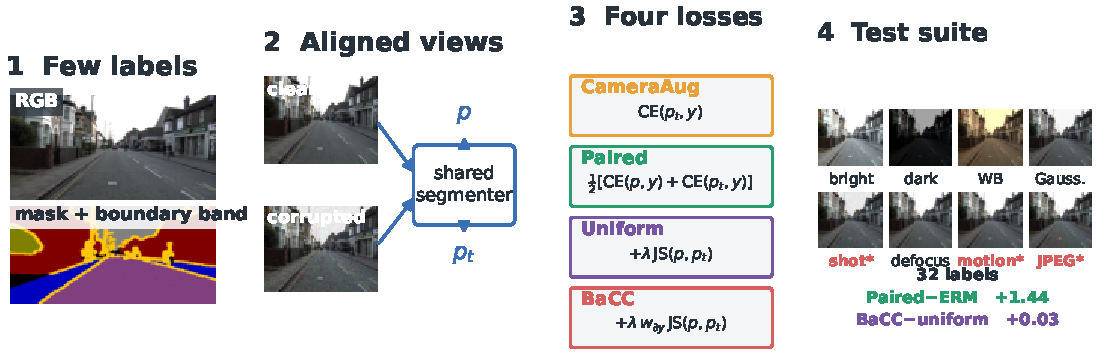
\includegraphics[width=\linewidth]{../results/aggregate/overview.pdf}
    \caption{\textbf{Protocol overview.} From 16--64 labeled road frames we
    make a camera-corrupted copy of every training image, pixel-aligned with
    the original (the boundary band used by \method{} is drawn under the
    mask). Both views pass through the same network, giving the two
    predictions $p$ and $p_t$ that the four losses combine. The test suite spans eight corruption families at three severities;
    red asterisks mark the three held-out families. At 32 labels, supervising
    the image together with its corrupted copy is worth $+1.44$ corruption mIoU
    (\miouc{}) over plain training; boundary-weighting the consistency term adds $+0.03$.}
    \label{fig:overview}
\end{figure}

\section{Introduction}

Road-scene segmentation is usually evaluated on clean images, but deployed
models sit behind cameras that misbehave: exposure overshoots, white balance
drifts, noise rises with gain, focus hunts, and compression discards what
remains. Corruptions of this kind cut segmentation accuracy
sharply~\cite{kamann2020benchmarking}, and foundation-scale models inherit the
weakness~\cite{schiappa2024robustness}.

Those studies train on thousands of densely labeled images; many projects
instead own a few dozen, because road video is cheap to record and slow to
label. Label-efficient segmentation has answers for clean accuracy: sparse
annotation~\cite{shin2021pixelpick}, strong
augmentation~\cite{yuan2021simple}, self-training~\cite{yang2022stpp},
weak-to-strong consistency~\cite{yang2023unimatch}. Those papers rarely
measure robustness, and the robustness literature in turn assumes full
supervision~\cite{kamann2020benchmarking} or specialized
synthesis~\cite{rubab2026safedrive}. It remains unclear which cheap training
choices help under camera corruption when only a few dozen frames are labeled,
and whether the gains extend to corruptions the training pipeline never
produced.

This paper builds that comparison, with nested label budgets of 16, 32, and 64
CamVid frames and a test suite of eight camera-corruption families at three
severities, three of which never appear during training. The baseline is
plain supervised training, i.e., empirical risk minimization (ERM):
cross-entropy on the labeled frames, with horizontal flips as the only
augmentation. From there we change one ingredient at a time. First we corrupt
the training images, either with generic color jitter (contrast and saturation
changes with no camera model behind them) or with the same kinds of
transformations a real camera produces (we call the latter camera
augmentation). Next we supervise each labeled frame together with its
corrupted copy; we call the two inputs the clean and corrupted views of the
frame, and this setting paired supervision. Finally we add a consistency loss
between the two predictions, uniform over pixels at first and then reweighted
toward semantic boundaries (\cref{fig:overview}).

The boundary-weighted variant is the one we propose, Boundary-Aware Camera
Consistency (\method{}). It targets a familiar dense-prediction failure:
corruption hurts most near thin structures and class transitions, while an
image-wide consistency average is dominated by easy interiors such as road and
sky. \method{} therefore shifts consistency weight into a narrow band around
ground-truth boundaries, with no new parameters and no inference cost. Boundary weighting
turned out to add very little: \method{}'s corruption mIoU stays within 0.24
points of uniform consistency at every budget, and its one reliable effect is a small
boundary-quality gain at 32 labels. The larger share of the improvement comes
from paired supervision.

Concretely, we contribute (i) a reproducible small-label robustness protocol
on CamVid with fixed nested splits and held-out corruption families;
(ii) evidence that paired supervision with camera-style corruption improves
corrupted-image accuracy at every budget and transfers to unseen families; and
(iii) a controlled negative result for boundary-weighted consistency against a
baseline that differs from it by exactly one term.

\section{Related Work}

\paragraph{Robust semantic segmentation.}
Kamann and Rother~\cite{kamann2020benchmarking} benchmarked segmentation under
a broad corruption suite and found noise, weather, and compression especially
damaging; a later analysis reached the same conclusion for foundation
segmentation models~\cite{schiappa2024robustness}. Remedies include
physics-based rain rendering~\cite{halder2019rain}, class-centric motion-blur
augmentation~\cite{aakanksha2023motionblur}, and diffusion-synthesized adverse
weather~\cite{rubab2026safedrive}; all assume abundant labels or a synthesis
pipeline. Our protocol instead uses tens of labels, no generator, and several
mundane camera failures.

\paragraph{Segmentation from few labels.}
PixelPick shows that a few well-chosen labeled pixels go a long
way~\cite{shin2021pixelpick}. Semi-supervised methods exploit unlabeled images
through strong augmentation~\cite{yuan2021simple}, uncertainty-guided
co-training~\cite{fan2022ucc}, selective self-training~\cite{yang2022stpp},
and weak-to-strong perturbations~\cite{yang2023unimatch}; MatchMask fine-tunes
a diffusion model to synthesize image--mask pairs~\cite{lin2026matchmask}. Our
setting is stricter: a fixed subset of frames provides all supervision, and the
question is robustness rather than clean accuracy.

\paragraph{Consistency and boundaries.}
Consistency under augmentation is a strong tool for
adaptation~\cite{araslanov2021augmentation}, though consistency under
low-level perturbations alone does not guarantee invariance to higher-level
change~\cite{lai2021directional}. Gated-SCNN showed that modeling boundaries
explicitly helps segmentation~\cite{takikawa2019gatedscnn}. \method{} borrows
the intuition without the
architecture: a ground-truth boundary band reweights a consistency loss.

\section{Method}

\subsection{Problem setting}

We are given $\mathcal{D}_L=\{(x_i,y_i)\}_{i=1}^{L}$ with
$L\in\{16,32,64\}$ RGB driving frames and dense labels over the $C=11$
standard CamVid classes (\cref{sec:protocol}). A network $f_\theta$ produces
logits $z=f_\theta(x)$ and probabilities $p=\operatorname{softmax}(z)$. We
model camera degradation as a family $\mathcal{T}$ of \emph{label-preserving}
transformations: every $t\in\mathcal{T}$ changes pixel values (brightness,
color balance, noise, blur, compression) but moves no pixels, so the
annotation of $x$ is also the annotation of $t(x)$, and a corrupted copy of a
labeled frame is supervised at no labeling cost.

\subsection{Camera corruptions: four for training, eight for testing}
\label{sec:corruptions}

During training, each batch draws one of four transformations: an
exposure/gamma shift (which may brighten or darken), a channel-wise
white-balance shift, additive Gaussian noise, or defocus blur, with severity
drawn from a continuous range, so the model does not train on the exact test
severities. We apply horizontal flips identically to both views and the mask.

At test time we fix every corruption: eight families (brightness, darkness,
white balance, Gaussian noise, shot noise, defocus blur, motion blur, and JPEG)
at three severity levels each (mild, moderate, severe), for 24 conditions in
total. Five of the eight correspond to the four training transformations,
since brightness and darkness are both exposure shifts. The remaining three
(shot noise, motion blur, JPEG) are never produced by the training pipeline;
we report them separately as \emph{held-out} families. Darkness runs past the training range: its
severe setting combines a strong gamma with a gain cut, leaving it darker than
any exposure shift the training pipeline produces. The augmented models pay
for that in \cref{sec:corruption-results}.

\subsection{Boundary-Aware Camera Consistency}

For a labeled image $x$ we compute predictions $p$ and $p_t$ for the clean
view and a corrupted view $t(x)$. Both views receive weighted cross-entropy:
\begin{equation}
\mathcal{L}_{\mathrm{sup}} = \tfrac{1}{2}\operatorname{CE}(f_\theta(x),y)
 + \tfrac{1}{2}\operatorname{CE}(f_\theta(t(x)),y),
\label{eq:sup}
\end{equation}
with inverse square-root class weights estimated only from the selected
labeled subset and clipped for stability.

To focus the consistency term, we mark every horizontal and vertical label
transition in $y$ and dilate the marks by radius $r$ into a boundary band
$b(y)$ (drawn under the mask in \cref{fig:overview}); ignored pixels are
excluded. We normalize the pixel weights so the loss keeps the same overall scale for
any band strength $\alpha$:
\begin{equation}
w_j = \frac{1+\alpha b(y)_j}
{\frac{1}{|\Omega|}\sum_{k\in\Omega}(1+\alpha b(y)_k)},
\label{eq:weight}
\end{equation}
where $\Omega$ is the set of valid pixels. Raising $\alpha$ moves consistency
weight from interiors to boundaries instead of growing the loss. We compare the two predictive distributions per pixel with the
Jensen--Shannon divergence
$\operatorname{JS}(p\,\|\,q)=\tfrac{1}{2}\operatorname{KL}(p\,\|\,m)
+\tfrac{1}{2}\operatorname{KL}(q\,\|\,m)$, $m=\tfrac{1}{2}(p+q)$, a symmetric
and bounded relative entropy. The labels supply all supervision through
\cref{eq:sup}; this term only asks the two predictions to agree, so neither is
a target for the other. The consistency loss is
\begin{equation}
\mathcal{L}_{\mathrm{BaCC}} = \frac{1}{|\Omega|}\sum_{j\in\Omega}
w_j\operatorname{JS}(p_j\,\|\,p_{t,j}),
\label{eq:bacc}
\end{equation}
and the objective is
$\mathcal{L}=\mathcal{L}_{\mathrm{sup}}+\lambda\mathcal{L}_{\mathrm{BaCC}}$.
Setting $\alpha=0$ recovers uniform consistency exactly.

We set $\alpha=3$ and the 400-update schedule from one pilot run at 32 labels,
before the main grid. \Cref{sec:ablation} sweeps $\alpha$ afterwards. The
radius $r=2$ gives a band a few pixels wide, comparable to the two-pixel
tolerance of the boundary-F1 metric, and we leave $\lambda=1$ because
\cref{eq:weight} already normalizes the consistency term. The same values apply
at every budget.

\section{Experimental Protocol}
\label{sec:protocol}

\paragraph{Dataset and label budgets.}
CamVid provides densely labeled frames from driving
video~\cite{brostow2009camvid}. We use the split popularized by
SegNet~\cite{badrinarayanan2017segnet}: 367 training, 101 validation, and 233
test frames, with the common 11-class mapping (road, building, car,
pedestrian, and so on) and an ignored void class. We resize every frame to
$288\times384$. For each of three seeds we draw one random
permutation of the training indices; its first 16, 32, and 64 entries form the
three nested budgets. No unlabeled data enters the comparison.

\paragraph{Model and optimization.}
The main architecture is DeepLabV3~\cite{chen2017deeplab} with an
ImageNet-pretrained MobileNetV3 backbone~\cite{howard2019mobilenetv3} and a
new 11-class head. Every method trains for 400 AdamW updates at batch
size 8 and keeps the checkpoint with the best clean validation mIoU. All
methods share the same batches, schedule, and pretrained initialization, and
differ only in augmentation and loss; the supplementary lists the remaining
optimizer settings. A secondary experiment swaps the decoder for Lite Reduced Atrous Spatial
Pyramid Pooling (LR-ASPP), a lighter segmentation head introduced with
MobileNetV3~\cite{howard2019mobilenetv3}.

\paragraph{Baselines.}
\emph{ERM} is the plain supervised baseline (cross-entropy, horizontal flips
only). \emph{ColorJitter} replaces each training image with a generically
jittered version (contrast and saturation). \emph{CameraAug} instead replaces
it with a camera-corrupted version drawn from \cref{sec:corruptions}. \emph{Paired} supervises the clean image and its
corrupted copy together (\cref{eq:sup}); the copy is generated on the fly at
each step, so the budget still holds $L$ distinct labeled frames.
\emph{Uniform consistency} adds an unweighted Jensen--Shannon consistency loss
between the two predictions. \emph{\method{}} uses the boundary-weighted
version of that loss. We train the six recipes separately and never
combine them: none applies both jitter and camera corruption, and a training
step uses at most two versions of a frame.

\paragraph{Metrics.}
We report clean-image mean intersection-over-union (mIoU); corruption mIoU
(\miouc{}), the average over all 24 corrupted conditions; held-out \miouc{}
over the nine held-out conditions; and class-agnostic boundary F1 at a
two-pixel tolerance, averaged over corrupted conditions. The supplementary
adds worst-family mIoU, expected calibration error (ECE), and per-class
results. All values are percentages and differences are percentage points.
Aggregates are three-seed means with 95\% $t$-intervals; with $n=3$ we lean on
effect sizes and per-seed wins and treat every paired test as exploratory.

\section{Results}

\subsection{Main comparison}

\IfFileExists{../results/aggregate/table_main.tex}{
\begin{table}[t]
\centering
\caption{Main CamVid results: mean $\pm$ 95\% $t$-interval over three nested-subset seeds (boundary F1: mean only). Bold marks the best value per column within each label budget; rounded ties share the bold. Worst-family mIoU and calibration for the same runs are tabulated in the supplementary.}
\label{tab:main}
\small
\setlength{\tabcolsep}{4.5pt}
\begin{tabular}{clrrrr}
\toprule
Labels & Method & Clean & \miouc{} & Held-out & Bnd.\ F1 \\
\midrule
\multirow{6}{*}{16} & ERM & 37.5 $\pm$ 4.5 & 33.6 $\pm$ 2.4 & 32.2 $\pm$ 1.0 & 27.2 \\
 & ColorJitter & 37.7 $\pm$ 4.8 & 33.6 $\pm$ 4.0 & 32.1 $\pm$ 3.0 & 27.8 \\
 & CameraAug & 37.9 $\pm$ 3.3 & 34.1 $\pm$ 5.5 & 33.6 $\pm$ 5.9 & \textbf{29.9} \\
 & Paired CameraAug & 38.1 $\pm$ 4.2 & \textbf{34.9} $\pm$ 3.6 & \textbf{34.1} $\pm$ 3.3 & \textbf{29.9} \\
 & Uniform consistency & \textbf{38.4} $\pm$ 3.6 & \textbf{34.9} $\pm$ 3.7 & \textbf{34.1} $\pm$ 3.7 & 29.5 \\
 & BaCC & 38.1 $\pm$ 3.7 & 34.7 $\pm$ 2.1 & \textbf{34.1} $\pm$ 2.8 & 29.6 \\
\midrule
\multirow{6}{*}{32} & ERM & 41.7 $\pm$ 1.2 & 37.3 $\pm$ 2.3 & 35.5 $\pm$ 3.0 & 29.5 \\
 & ColorJitter & 41.8 $\pm$ 3.8 & 37.3 $\pm$ 3.7 & 35.6 $\pm$ 4.5 & 30.6 \\
 & CameraAug & 41.8 $\pm$ 0.5 & 37.7 $\pm$ 1.8 & 37.2 $\pm$ 1.6 & 32.0 \\
 & Paired CameraAug & \textbf{42.9} $\pm$ 1.1 & \textbf{38.8} $\pm$ 0.5 & \textbf{37.9} $\pm$ 1.2 & 32.3 \\
 & Uniform consistency & 42.6 $\pm$ 1.5 & 38.7 $\pm$ 1.0 & \textbf{37.9} $\pm$ 1.4 & 32.0 \\
 & BaCC & 42.8 $\pm$ 1.8 & 38.7 $\pm$ 1.8 & \textbf{37.9} $\pm$ 2.0 & \textbf{32.7} \\
\midrule
\multirow{6}{*}{64} & ERM & 46.4 $\pm$ 3.4 & 41.0 $\pm$ 2.9 & 38.7 $\pm$ 3.1 & 32.6 \\
 & ColorJitter & 46.1 $\pm$ 5.2 & 41.0 $\pm$ 3.6 & 38.8 $\pm$ 3.5 & 32.5 \\
 & CameraAug & \textbf{46.8} $\pm$ 1.6 & 42.1 $\pm$ 3.2 & \textbf{41.6} $\pm$ 3.3 & 34.4 \\
 & Paired CameraAug & 46.5 $\pm$ 2.8 & 42.1 $\pm$ 2.8 & 41.0 $\pm$ 2.6 & \textbf{34.6} \\
 & Uniform consistency & 46.7 $\pm$ 2.6 & \textbf{42.4} $\pm$ 2.6 & 41.4 $\pm$ 2.4 & 34.4 \\
 & BaCC & 46.6 $\pm$ 2.4 & \textbf{42.4} $\pm$ 2.4 & 41.4 $\pm$ 2.3 & 34.4 \\
\bottomrule
\end{tabular}
\end{table}

}{\todo{Run camrobust-analyze to generate Table 1.}}

Label count matters more than any training choice we tested
(\cref{tab:main}, \cref{fig:diagnostics}). ERM alone goes from 33.6 \miouc{}
at 16 labels to 37.3 at 32 and 41.0 at 64, a swing wider than the spread
between methods at any single budget. ColorJitter scores the same \miouc{} as ERM
at all three budgets (33.6, 37.3, 41.0), so augmentation appears to pay only
when it resembles the corruption it has to survive. The camera-aware variants do
help, and most of the gain appears once both views are supervised. At
32 labels Paired reaches 38.8 \miouc{}, 1.44 above ERM, and beats CameraAug on
all three seeds (mean $+1.03$, exploratory paired $p=0.076$). Uniform
consistency then adds at most 0.31 points at any budget, and it edges ahead at
64 labels (42.4) by 0.31 over Paired. Intervals at 16 labels are wide enough
that we would not rank methods on a single subset.

\begin{figure}[t]
    \centering
    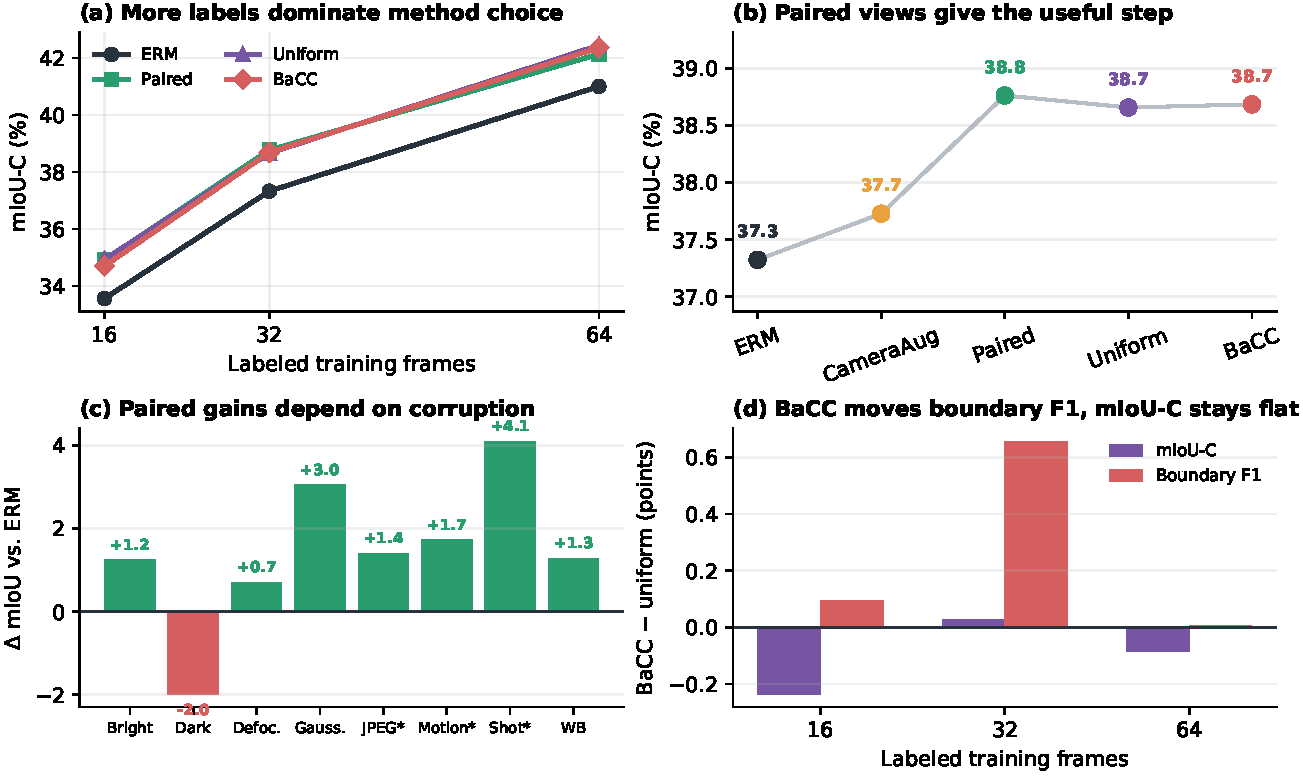
\includegraphics[width=0.82\linewidth]{../results/aggregate/diagnostics.pdf}
    \caption{\textbf{Where the gains come from.} (a) Camera-aware variants
    separate from ERM as labels grow. (b) At 32 labels the useful step is
    supervising both views. (c) Paired$-$ERM per family at 32 labels: strong
    transfer to held-out shot noise and motion blur (asterisks), a regression
    on darkness. (d) \method{}$-$Uniform at each budget: boundary F1 responds
    at 32 labels while \miouc{} stays flat. Three-seed means throughout.}
    \label{fig:diagnostics}
\end{figure}

\subsection{Corruption-level and boundary analysis}
\label{sec:corruption-results}

Held-out corruptions transfer better than we expected. At 32 labels, CameraAug
lifts held-out \miouc{} from 35.5 to 37.2; Paired reaches 37.9. The largest
single transfer is shot noise, never seen in training: 30.9 for ERM versus
35.3 for Uniform consistency. Motion blur and JPEG improve too
(\cref{fig:diagnostics}c): training against Gaussian noise evidently carries
over to other sensor noise and even to compression. At 64 labels CameraAug beats ERM on held-out \miouc{} by
2.93 points on every seed (exploratory $p=1.2\times10^{-4}$).

Darkness is the exception: ERM scores 38.0 there, CameraAug 33.0, Uniform
consistency 35.6. As anticipated in \cref{sec:corruptions}, the severe test
darkness lies outside the training exposure range, and models that leaned on
that augmentation do worse than a model trained without it. Augmentation helps
up to the edge of the conditions it actually produces, and can hurt beyond it.

Boundary quality follows accuracy: CameraAug raises corrupted boundary F1 over
ERM by 2.72, 2.48, and 1.80 points at the three budgets. \method{}'s boundary
weighting adds 0.66 F1 over Uniform consistency at 32 labels (on two of three
seeds) while moving \miouc{} by $+0.03$ ($p=0.93$): it improves the boundary
metric it was designed for, at one budget, without moving accuracy. ECE shows no consistent
pattern across budgets (supplementary); robustness gains do not imply
calibration gains. \Cref{fig:qualitative} shows what these deltas look like on
real frames.

\begin{figure}[t]
    \centering
    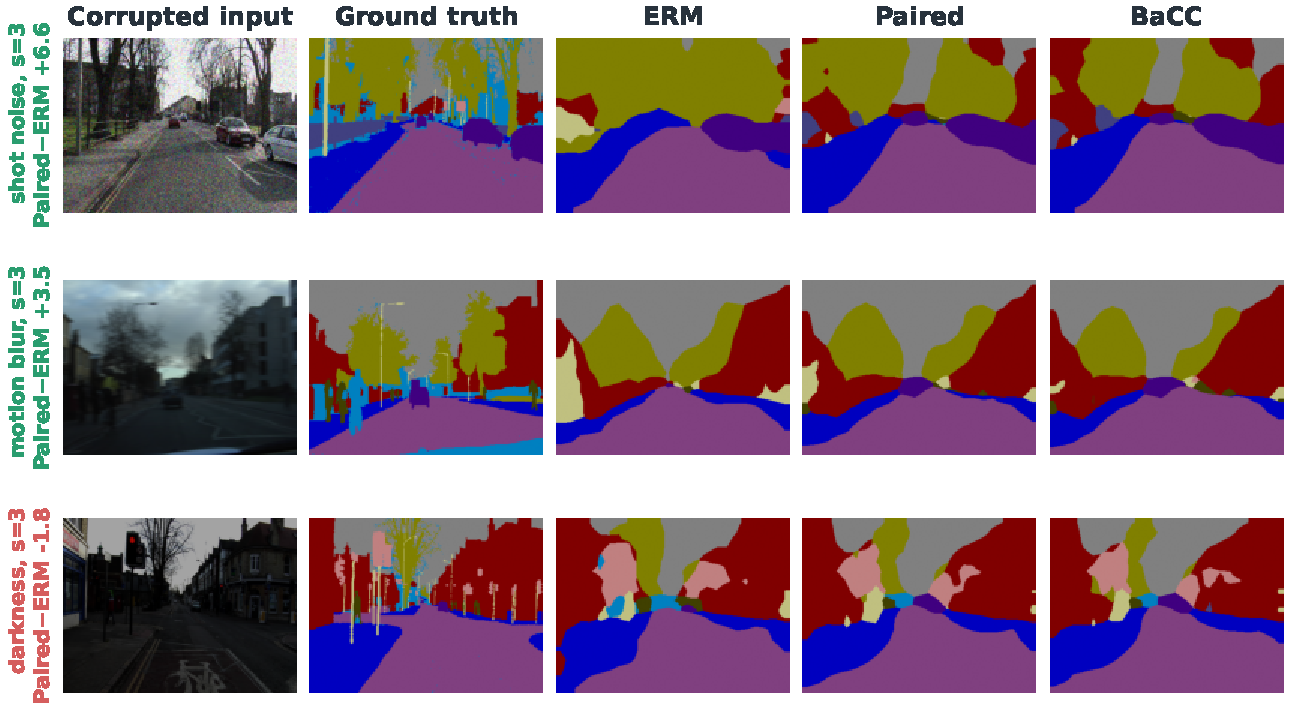
\includegraphics[width=0.82\linewidth]{../results/aggregate/qualitative_main.pdf}
    \caption{\textbf{What the deltas look like.} Median per-image Paired$-$ERM
    improvement under held-out shot noise and motion blur, and the median
    regression under darkness, chosen by a fixed rule over the full test split
    before viewing predictions (per-image mIoU, seed-0 checkpoints; aggregate
    claims rest on \cref{tab:main}). Paired training keeps road and vehicle
    structure under noise and blur; under severe darkness every model
    degrades.}
    \label{fig:qualitative}
\end{figure}

\subsection{Ablations and architecture transfer}
\label{sec:ablation}

Sweeping the boundary weight $\alpha\in\{0,1,3,6\}$ at 32 labels moves
\miouc{} only within 38.6--38.9; $\alpha=3$ gives the best boundary F1 (32.7)
but not the best accuracy (supplementary ablation table). The sweep is flat: the
improvement comes from the paired views, and the exact boundary weight barely
matters. We can only conjecture why
the reweighting does so little. Because \cref{eq:weight} holds the total
consistency budget fixed, a larger $\alpha$ buys boundary weight by taking it
from interior pixels, and with a few dozen frames those interiors still supply
most of the signal the model can use.

Swapping DeepLabV3 for LR-ASPP reproduces the effect: the full \method{} recipe
improves \miouc{} from 36.1 to 38.6 and held-out \miouc{} from 33.1 to 36.7
over ERM. This check compares complete recipes, so it shows camera-aware
training transferring across decoders without isolating the boundary term.

\section{Limitations and Conclusion}

Most of these limits come with the small-label regime. CamVid is small, captured in one English city, and temporally
correlated, so three subset seeds quantify how much the choice of frames
matters and say little about other countries, sensors, or weather. At 16--64
labels that choice is itself a major source of variance, which is why we
report per-seed values and treat the paired tests as exploratory. Our
corruptions are controlled models of camera failure (JPEG is real codec
output; the noise and blur are simplified), which is standard for corruption
benchmarks. \method{} needs dense labels to build its boundary band, so it does not
extend to image-level tags or scattered labeled pixels.

With 16--64 labeled road frames, the recipe our study supports is short: make
a camera-corrupted copy of each labeled frame and supervise both together.
Uniform consistency and boundary weighting moved corruption mIoU by fractions
of a point at these budgets, and the gains stop where augmentation coverage
stops, as darkness shows. We release the
code, the fixed splits, and all 66 run records.

\bibliographystyle{splncs04}
\bibliography{references}

\end{document}
